\documentclass[french]{article}

\usepackage{mathtools, bm}
\usepackage{amssymb, bm}
\usepackage[utf8]{inputenc}
\usepackage[T1]{fontenc}
\usepackage{babel}
\usepackage{amsmath}
\usepackage{graphicx}
\usepackage{eso-pic}
\usepackage{fullpage}
\usepackage{ulem}
\usepackage{ntheorem}
\usepackage{xcolor}
\usepackage{titlesec}
\usepackage{stmaryrd}
\usepackage{calrsfs}
\usepackage{textcomp}
\usepackage[left=2cm,right=2cm,top=2cm,bottom=2cm]{geometry}
\theorembodyfont{\upshape}
\theoremstyle{break}

\definecolor{rougetitre}{RGB}{240, 23, 23}
\definecolor{dorure}{RGB}{147, 127, 8}
\definecolor{dorure2}{RGB}{135, 100, 6}
\definecolor{dorure3}{RGB}{102, 68, 0}
\definecolor{bleuturquoise}{RGB}{30, 81, 122}
\definecolor{vertturquoise}{RGB}{15, 127, 110}
\definecolor{fond}{RGB}{240,240,240}

\titleformat{\section}
   {}% apparence commune au titre et au numéro
   {}% apparence du numéro
   {1em}% espacement numéro/texte
   {\LARGE}% apparence du titre

\titleformat{\subsection}
   {}% apparence commune au titre et au numéro
   {}% apparence du numéro
   {1em}% espacement numéro/texte
   {\large}% apparence du titre

\titleformat{\subsubsection}
   {}% apparence commune au titre et au numéro
   {}% apparence du numéro
   {1em}% espacement numéro/texte
   {\underline}% apparence du titre

\title{Projet base de données}
\author{Julie SAOULI, Maxime GOURGOULHON, Pierre BOUVIER, Geoffrey TANGUY, Jérôme THÉATE}
\date{ENSIMAG | Enseignant encadrant : M. Christophe BOBINEAU | 2017 - 2018 }
\makeatletter 
\begin{document}
\renewcommand*\contentsname{\huge{Table des matières\vspace{1cm}}}
\begin{titlepage}
\begin{center}
\text{  }\\
\text{  }\\
\text{  }\\
\text{  }\\
\textcolor{dorure3}{\textbf{{\fontsize{45}{45}\selectfont Projet Base de Données}}}\\
\vspace{0.5cm}
\textcolor{dorure3}{\textbf{\LARGE{COMPTE-RENDU}}}
\end{center}
\vspace{3cm}
\begin{center}
\makebox[\textwidth]{\includegraphics[scale = 1, width=\paperwidth,height=10cm]{proverbe2.jpg}}
\end{center}

\vspace{4.0cm}
\begin{center}
Julie SAOULI \hspace{1.5cm} Maxime GOURGOULHON  \hspace{1.5cm} Pierre BOUVIER
\end{center}
\\
\hspace{4.2cm} Geoffrey TANGUY \hspace{3cm} Jérôme THÉATE
\\
\vspace{0.2cm}
\begin{center}
\large{\@date}
\end{center}
\end{titlepage}
\clearpage

\begin{Large}
\tableofcontents{}
\end{Large}
\clearpage







\textsc{\textcolor{dorure2}{\LARGE{Introduction}}}
\addcontentsline{toc}{section}{Introduction}
\vspace{1cm}

L'agence de voyage \textsc{awhy}, forte de son succès, entreprend sa transformation numérique.

Elle tient à numériser ses outils de gestion : CRM, suivi de voyage, etc., et base de données. Tout en concervant une étroite collaboration avec ses entreprises partenaires. De ce fait, certaines règles d'implémentation devront être respectées afin d'assurer le fonctionnement des outils numériques entre tous les partenaires.\\

Dans le cadre du développement de la société \textsc{awhy}, nous avons été mendaté afin de réaliser la conception et l'implémentation de leur base de données. Ce rapport vous apportera les outils necessaires à la compréhension de la conception de cette base de données. Et vous permettra en outre de prendre connaissance des enjeux et des difficultés qui ont permis de privilégier certains axes de réflexion.
Enfin, vous y trouverez certains détails quant à nos choix d'implémentation, nous permettant de mettre en valeur et d'exploiter le potentiel de la base de données.










\noindent\textsc{\textcolor{dorure2}{\section{Conception de la base de données}}}

\textsc{\textcolor{dorure}{\subsection{Propriétés élémentaires}}}
\vspace{0.3cm}

\{ nomVille, pays, nomLieu, adresseLieu, descriptifLieu, prix,
idCircuit, descriptif, villeDépart, paysDepart, villeArrivee, paysArrivee, nbJoursTotal, prixCircuit, dateDepartCircuit, nbPersonnes, ordre, nbJours, nomHotel, adresseHotel, nbChambresTotal, prixChambre, prixPetitDejeuner, numDossier, idClient, typeClient, anneeEnregistrement, nomClient, prenomClient, adresseClient, emailClient, telClient, datePaiement, infoPaiement, nbChambres, dateDepartHotel, dateArriveeHotel, dateVisite, nbPersonnesVisite, nbChambresReservees, nbPetitDejReserves, numDossierReservation \}




\vspace{0.3cm}
\textsc{\textcolor{dorure}{\subsection{Dépendances fonctionnelles}}}
\vspace{0.3cm}





\textsc{Issues du sujet :}
\vspace{0.3cm}

\begin{small}
\noindent nomLieu, nomVille, pays → adresseLieu, descriptifLieu, prix\\
\noindent idCircuit → descriptif, villeDepart, paysDepart, villeArrivee, paysArrivee, nbJoursTotal, prixCircuit\\
idCircuit, dateDepartCircuit → nbPersonnes\\
idCircuit, ordre → nomLieu, nomVille, pays, nbJours\\
nomHotel, nomville, pays → adresseHotel, nbChambresTotal, prixChambre, prixPetitDejeuner\\
\end{small}

\textsc{Issues de notre sgbd:}
\vspace{0.3cm}

\begin{small}
\noindent idClient → nomClient, prenomClient, typeClient, adresseClient, emailClient, telClient, annéeEnregistrement\\
numDossier, idCircuit, dateDepartCircuit → nbPersonnesCircuit\\
villeDepart, paysDepart → nomVille, pays\\
villeArrivee, paysArrivee → nomVille, pays\\
numDossier, nomHotel, nomVille, pays, dateDepartHotel, dateArriveeHotel → nbChambresReservees, nbPetitDejReserves\\
numDossier, nomLieu, nomVille, pays, dateVisite → nbPersonnesVisite\\
numDossierReservation → datePaiement, infoPaiement\\
numDossierReservation → idClient
\end{small}




\vspace{0.3cm}
\textsc{\textcolor{dorure}{\subsection{Contraintes de multiplicité}}}
\vspace{0.3cm}




\noindent numDossier $-|\twoheadrightarrow$ nomHotel, nomVille, pays\\
nomHotel, nomVille, pays $-|\twoheadrightarrow$ numDossier\\
numDossier $-|\twoheadrightarrow$ nomLieu, nomVille, pays\\
nomLieu, nomVille, pays $-|\twoheadrightarrow$ numDossier\\
numDossier, dateDepartHotel, dateArriveeHotel $\twoheadrightarrow$ nomHotel, nomVille, pays\\
nomHotel, nomVille, pays, dateDepartHotel, dateArriveeHotel $\twoheadrightarrow$ numDossier\\
numDossier, dateVisite $\twoheadrightarrow$ nomLieu, nomVille, pays\\
nomLieu, nomVille, pays, dateVisite $\twoheadrightarrow$ numDossier\\
numDossier $-|\twoheadrightarrow$ idCircuit, dateDepartCircuit\\
idCircuit, dateDepartCircuit $-|\twoheadrightarrow$ numDossier\\
idClient $\twoheadrightarrow$ numDossierReservation\\
idCircuit $\twoheadrightarrow$ idCircuit, dateDepartCircuit\\
nomVille, pays $-|\twoheadrightarrow$ nomLieu, nomVille, pays\\
nomVille, pays $-|\twoheadrightarrow$ nomHotel, nomVille, pays\\
nomLieu, nomVille, pays $-|\twoheadrightarrow$ idCircuit, ordre\\
nomVille, pays $-|\twoheadrightarrow$ villeDepart, paysDepart\\
nomVille, pays $-|\twoheadrightarrow$ villeArrivee, paysArrivee




\vspace{0.3cm}
\textsc{\textcolor{dorure}{\subsection{Contraintes autres}}}
\vspace{0.3cm}




\noindent “Un dossier contient au moins une réservation (hôtel, circuit, lieux).”\\
“Il ne peut y avoir deux villes de même nom dans le même pays.”\\
“Un circuit commence par une étape de départ et se termine par une étape d’arrivée. Tout circuit contient au moins deux étapes : le départ et l’arrivée.”\\
“Un client doit avoir au moins une réservation (simulation payée).”\\
“Au paiement, et pour permettre la réservation du voyage, il faut vérifier la disponibilité des hôtels et circuits réservés (nombre de places libres compatible avec nombre de places réservées) ainsi que toutes les contraintes.”





\vspace{0.3cm}
\textsc{\textcolor{dorure}{\subsection{Schéma Entité/Association}}}
\vspace{0.3cm}





\begin{center}
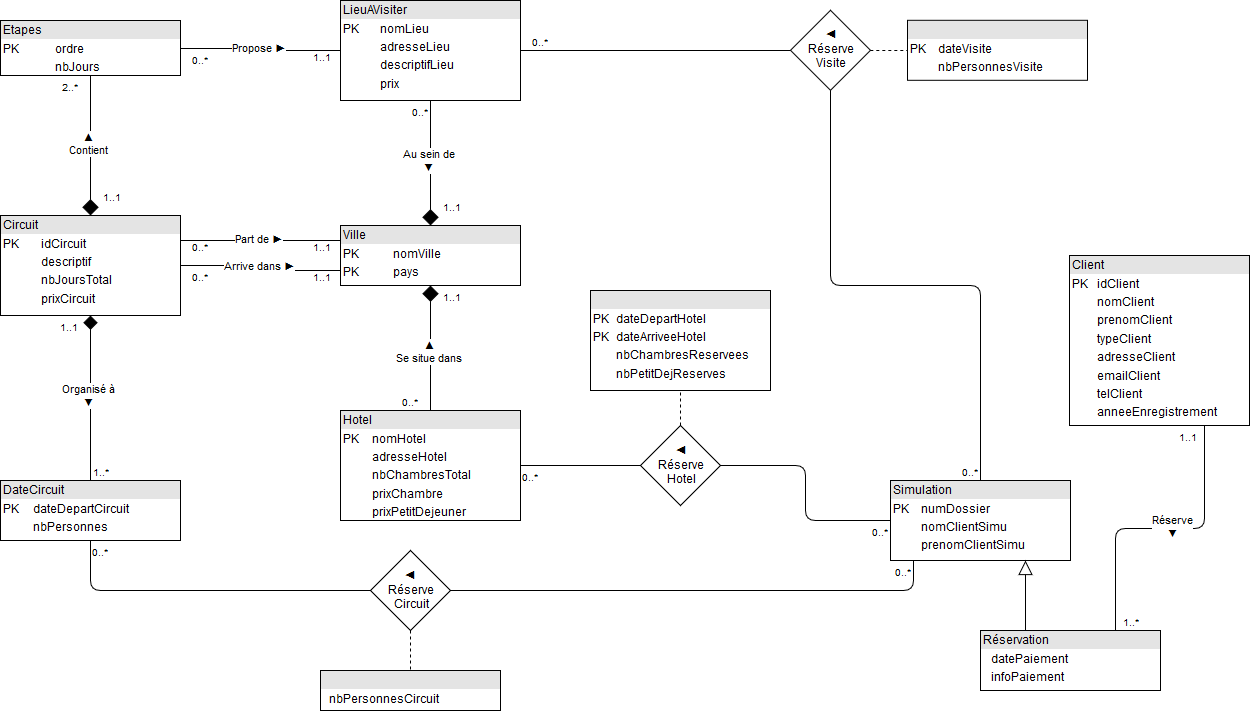
\includegraphics[scale = 0.4]{schema_uml.jpg}
\end{center}

\end{document}
